\documentclass[tikz]{standalone}
\usepackage{tikz}
\usepackage{bm}
\usetikzlibrary{decorations.pathreplacing,arrows}

\begin{document}
\boldmath

	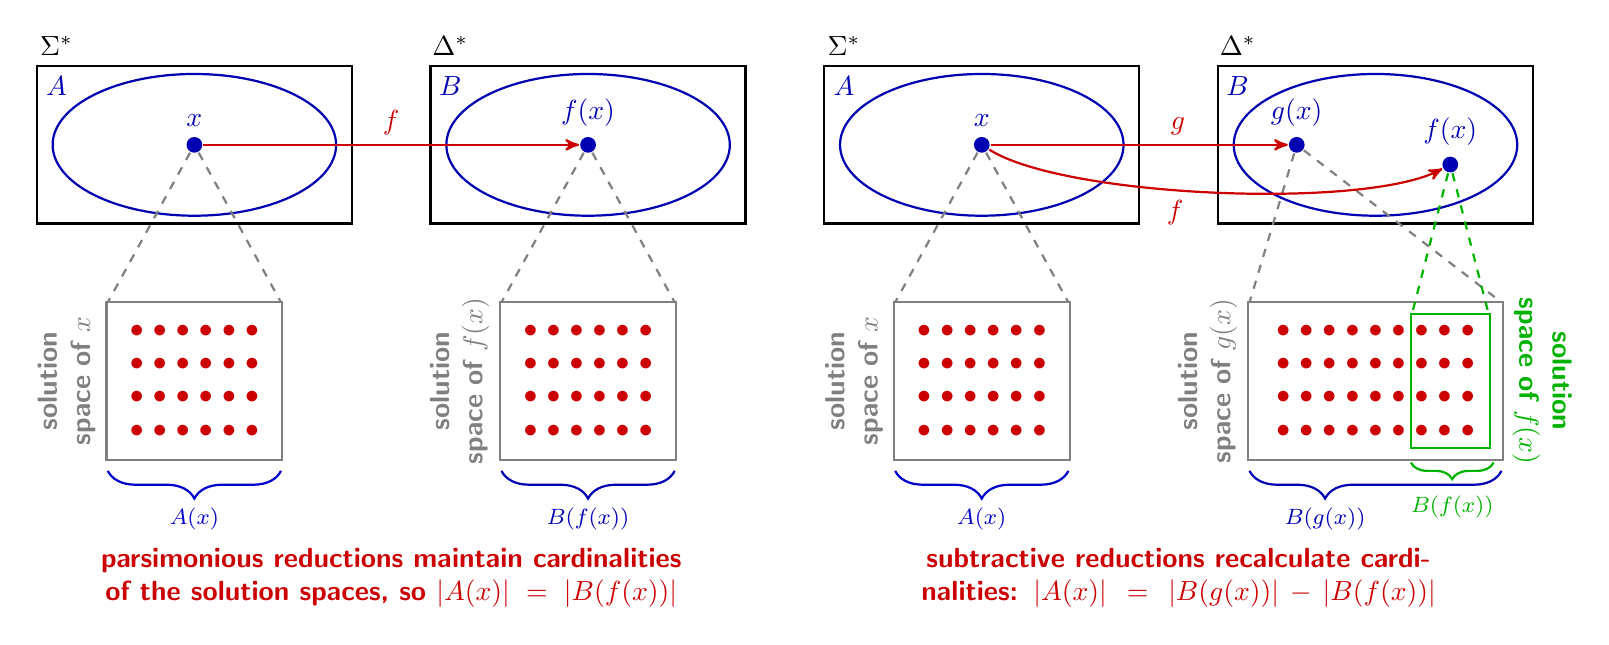
\begin{tikzpicture}
	
	%% Start Parsimonious Case
		% Sigma*
		\node at (0.25,2.25) {$\Sigma^*$};
		\draw[thick] (0,0) rectangle (4,2);
		
		% A
		\node[blue!70!black] at (0.25,1.75) {$A$};
		\draw[thick,blue!70!black] (2,1) ellipse (1.8cm and .9cm);
		
		% x
		\node[circle,thick,fill=blue!70!black,inner sep=0mm,minimum width=2mm,label={90:\color{blue!70!black}$x$}] (x) at (2,1) {};
		
		% Solution space of x
		\node[thick,draw=gray,rectangle,minimum width=2cm,minimum height=2cm,text width=2cm,align=center,label={[text width=2cm,rotate=90,anchor=south,align=center]180:\sffamily\bfseries\color{gray}solution space of $x$}] at (2,-2) {\color{red!80!black}$\bullet$ $\bullet$ $\bullet$ $\bullet$ $\bullet$ $\bullet$\\$\bullet$ $\bullet$ $\bullet$ $\bullet$ $\bullet$ $\bullet$\\$\bullet$ $\bullet$ $\bullet$ $\bullet$ $\bullet$ $\bullet$\\$\bullet$ $\bullet$ $\bullet$ $\bullet$ $\bullet$ $\bullet$};
		
		% Dashed Lines to edges of solution space of x
		\path[thick,gray,dashed] 
			(x) edge (.9,-1)
			(x) edge (3.1,-1);
			
		% Curly Brace under solution space of x
		\draw [decorate,blue!80!black,thick,decoration={brace,amplitude=10pt,mirror,raise=4pt},yshift=0pt] (.9,-3) -- (3.1,-3) node [blue!80!black,midway,yshift=-.75cm] {\footnotesize $A(x)$};
		
		% Delta*
		\node at (5.25,2.25) {$\Delta^*$};
		\draw[thick] (5,0) rectangle (9,2);

		% B
		\node[blue!70!black] at (5.25,1.75) {$B$};
		\draw[thick,blue!70!black] (7,1) ellipse (1.8cm and .9cm);		

		% f(x)
		\node[circle,thick,fill=blue!70!black,inner sep=0mm,minimum width=2mm,label={90:\color{blue!70!black}$f(x)$}] (fx) at (7,1) {};
		
		% Solution space of f(x)
		\node[thick,draw=gray,rectangle,minimum width=2cm,minimum height=2cm,text width=2cm,align=center,label={[text width=2.5cm,rotate=90,anchor=south,align=center]180:\sffamily\bfseries\color{gray}solution space of $f(x)$}] at (7,-2) {\color{red!80!black}$\bullet$ $\bullet$ $\bullet$ $\bullet$ $\bullet$ $\bullet$\\$\bullet$ $\bullet$ $\bullet$ $\bullet$ $\bullet$ $\bullet$\\$\bullet$ $\bullet$ $\bullet$ $\bullet$ $\bullet$ $\bullet$\\$\bullet$ $\bullet$ $\bullet$ $\bullet$ $\bullet$ $\bullet$};
		
		% Dashed Lines to edges of solution space of f(x)
		\path[thick,gray,dashed] 
			(fx) edge (5.9,-1)
			(fx) edge (8.1,-1);

		% Curly Brace under solution space of f(x)
		\draw [decorate,blue!70!black,thick,decoration={brace,amplitude=10pt,mirror,raise=4pt},yshift=0pt] (5.9,-3) -- (8.1,-3) node [blue!70!black,midway,yshift=-.75cm] {\footnotesize $B(f(x))$};
		
		
		% Arrow from x to f(x)
		\path[thick,red!80!black,-stealth'] (x) edge [above] node {\color{red!80!black}$ f$} (fx);
		
		% Explanation
		\node[text width=9cm,font=\color{red!80!black}\bfseries\sffamily,align=center] at (4.5,-4.5) {parsimonious reductions maintain cardinalities of the solution spaces, so $|A(x)|=|B(f(x))|$};

	%%%%%%%%%%%%%%%%%%%%%%%%%%%%
	%% Start Subtractive Case %%
	%%%%%%%%%%%%%%%%%%%%%%%%%%%%
	\begin{scope}[xshift=10cm]
		% Sigma*
		\node at (0.25,2.25) {$\Sigma^*$};
		\draw[thick] (0,0) rectangle (4,2);
		
		% A
		\node[blue!70!black] at (0.25,1.75) {$A$};
		\draw[thick,blue!70!black] (2,1) ellipse (1.8cm and .9cm);
		
		% x
		\node[circle,thick,fill=blue!70!black,inner sep=0mm,minimum width=2mm,label={90:\color{blue!70!black}$x$}] (x) at (2,1) {};
		
		% Solution space of x
		\node[thick,draw=gray,rectangle,minimum width=2cm,minimum height=2cm,text width=2cm,align=center,label={[text width=2cm,rotate=90,anchor=south,align=center]180:\sffamily\bfseries\color{gray}solution space of $x$}] at (2,-2) {\color{red!80!black}$\bullet$ $\bullet$ $\bullet$ $\bullet$ $\bullet$ $\bullet$\\$\bullet$ $\bullet$ $\bullet$ $\bullet$ $\bullet$ $\bullet$\\$\bullet$ $\bullet$ $\bullet$ $\bullet$ $\bullet$ $\bullet$\\$\bullet$ $\bullet$ $\bullet$ $\bullet$ $\bullet$ $\bullet$};
		
		% Dashed Lines to edges of solution space of x
		\path[thick,gray,dashed] 
			(x) edge (.9,-1)
			(x) edge (3.1,-1);
			
		% Curly Brace under solution space of x
		\draw [decorate,blue!80!black,thick,decoration={brace,amplitude=10pt,mirror,raise=4pt},yshift=0pt] (.9,-3) -- (3.1,-3) node [blue!80!black,midway,yshift=-.75cm] {\footnotesize $A(x)$};
		
		% Delta*
		\node at (5.25,2.25) {$\Delta^*$};
		\draw[thick] (5,0) rectangle (9,2);

		% B
		\node[blue!70!black] at (5.25,1.75) {$B$};
		\draw[thick,blue!70!black] (7,1) ellipse (1.8cm and .9cm);		

		% g(x)
		\node[circle,thick,fill=blue!70!black,inner sep=0mm,minimum width=2mm,label={90:\color{blue!70!black}$g(x)$}] (gx) at (6,1) {};
		
		% f(x)
		\node[circle,thick,fill=blue!70!black,inner sep=0mm,minimum width=2mm,label={90:\color{blue!70!black}$f(x)$}] (fx) at (7.95,.75) {};
		
		% Solution space of g(x)
		\node[thick,draw=gray,rectangle,minimum width=3cm,minimum height=2cm,text width=3cm,align=center,label={[text width=2.5cm,rotate=90,anchor=south,align=center]180:\sffamily\bfseries\color{gray}solution space of $g(x)$}] at (7,-2) {\color{red!80!black}$\bullet$ $\bullet$ $\bullet$ $\bullet$ $\bullet$ $\bullet$ $\bullet$ $\bullet$ $\bullet$ $\bullet$ $\bullet$ $\bullet$ $\bullet$ $\bullet$ $\bullet$ $\bullet$ $\bullet$ $\bullet$ $\bullet$ $\bullet$ $\bullet$ $\bullet$ $\bullet$ $\bullet$ $\bullet$ $\bullet$ $\bullet$ $\bullet$ $\bullet$ $\bullet$ $\bullet$ $\bullet$ $\bullet$ $\bullet$ $\bullet$ $\bullet$ };
		
		% Solution space of f(x)
		\node[thick,draw=green!70!black,rectangle,minimum width=1cm,minimum height=1.7cm,align=center,label={[text width=2.5cm,rotate=270,anchor=south,align=center,yshift=1ex]0:\sffamily\bfseries\color{green!70!black}solution space of $f(x)$}] at (7.95,-2) {};
		
		% Dashed Lines to edges of solution space of g(x)
		\path[thick,gray,dashed] 
			(gx) edge (5.4,-1)
			(gx) edge (8.6,-1);

		% Dashed Lines to edges of solution space of f(x)
		\path[thick,green!70!black,dashed] 
			(fx) edge (7.45,-1.2)
			(fx) edge (8.45,-1.2);

		% Curly Brace under solution space of g(x)
		\draw [decorate,blue!70!black,thick,decoration={brace,amplitude=10pt,mirror,raise=4pt,aspect=0.3},yshift=0pt] (5.4,-3) -- (8.6,-3) node [blue!70!black,pos=.3,yshift=-.75cm] {\footnotesize $B(g(x))$};

		% Curly Brace under solution space of f(x)
		\draw [decorate,green!70!black,thick,decoration={brace,amplitude=6pt,mirror,raise=1pt},yshift=0pt] (7.45,-3) -- (8.5,-3) node [green!70!black,midway,yshift=-.6cm] {\footnotesize $B(f(x))$};
		
		% Arrow from x to f(x) and g(x)
		\path[thick,red!80!black,-stealth'] 
			(x) edge [above,pos=.63] node {\color{red!80!black}$g$} (gx)
			(x) edge [above,pos=.43,bend right,below,looseness=.5] node {\color{red!80!black}$f$} (fx);

		% Explanation
		\node[text width=9cm,font=\color{red!80!black}\bfseries\sffamily,align=center] at (4.5,-4.5) {subtractive reductions recalculate cardinalities: $|A(x)|=|B(g(x))|-|B(f(x))|$};
	\end{scope}


	\end{tikzpicture}
\end{document}